%% Template for MLP Coursework 2 / 6 November 2017 

%% Based on  LaTeX template for ICML 2017 - example_paper.tex at 
%%  https://2017.icml.cc/Conferences/2017/StyleAuthorInstructions

\documentclass{article}
\usepackage[T1]{fontenc}
\usepackage{amssymb,amsmath}
\usepackage{txfonts}
\usepackage{microtype}
\usepackage{xspace}
\xspaceaddexceptions{\%}

% Lists with less spacoing between items
\usepackage{paralist}

% For figures
\usepackage{graphicx}
\usepackage{subfig} 

% For citations
\usepackage{natbib}

% For algorithms
\usepackage{algorithm}
\usepackage{algorithmic}

% the hyperref package is used to produce hyperlinks in the
% resulting PDF.  If this breaks your system, please commend out the
% following usepackage line and replace \usepackage{mlp2017} with
% \usepackage[nohyperref]{mlp2017} below.
\usepackage[hyphens]{url}
\urlstyle{same}
\usepackage{hyperref}

% Packages hyperref and algorithmic misbehave sometimes.  We can fix
% this with the following command.
\newcommand{\theHalgorithm}{\arabic{algorithm}}


% Set up MLP coursework style (based on ICML style)
\usepackage{mlp2020}
\mlptitlerunning{MLP Coursework 2 (\studentNumber)}
\bibliographystyle{icml2017}


\DeclareMathOperator{\softmax}{softmax}
\DeclareMathOperator{\sigmoid}{sigmoid}
\DeclareMathOperator{\sgn}{sgn}
\DeclareMathOperator{\relu}{relu}
\DeclareMathOperator{\lrelu}{lrelu}
\DeclareMathOperator{\elu}{elu}
\DeclareMathOperator{\selu}{selu}
\DeclareMathOperator{\maxout}{maxout}







%% You probably do not need to change anything above this comment

%% REPLACE this with your student number
\def\studentNumber{sXXXXXXX}

\begin{document} 

\twocolumn[
\mlptitle{MLP Coursework 2: Investigating the Optimization of Convolutional Networks}

\centerline{\studentNumber}

\vskip 7mm
]

\begin{abstract} 
The abstract should be a few sentences (100--200 words) long,  providing a concise summary of the contents of your report including the key research question(s) addressed: Why the optimization of VGG38 models more challenging as compared to VGG08, how the quantitative evaluation of the problem helped in debugging?, the methods explored in the literature for solving this problem, how effectively your chosen/proposed solution helped in solving the problem, the data used, and the findings of the experiments. 


\end{abstract} 

\section{Introduction}
\label{sec:intro}
This document provides a template for the MLP coursework 2 report.  This template structures the report into sections, which you are recommended to use, but can change if you wish.  If you want to use subsections within a section that is fine, but please do not use any deeper structuring. In this template the text in each section will include an outline of what you should include in each section, along with some practical LaTeX examples (for example figures, tables, algorithms).  Your document should be no longer than \textbf{six pages},  with an additional page (or more!) allowed for references.

The introduction should place your work in context, giving the overall \textbf{motivation} for the work, and clearly outlining the \textbf{objectives} of the work and the \textbf{research questions} you have explored -- in this case the debugging of optimization problems in CNN architectures. The introduction should be \textbf{no longer than maximum of 600 words}. 

In a general setting, the introduction should start by briefly discussing about the research area (of interest in the report) as explored in the literature. Then, defining the problem setting that is being looked at in the report - more specifically how optimization varies from shallow to deeper CNN architectures. What is the problem you identified that affects the training in Figure 1 and how you diagnosed it. Briefly discuss this in your own words, the motivation behind looking at this research question and how you approached the problem. 

Summarize how you investigated and debugged the problem/research question being addressed. Are there any methods/solutions in the literature that have looked at similar research problems? How did you go about finding a solution to the research question posed? Discuss the objectives of your proposed method and the findings/hypothesis that you build empirically, theoretically and intuitively. Were your proposed solutions effective and what were your final takeaways from the experiments? 

Conclude the introduction by outlining your major improvements and contributions.



\section{Identifying training problems of a deep CNN}

This section should introduce the  part of the report that has to do with identifying the given optimization problem in deep neural networks, and the ways of diagnosing and visualizing it. State clearly what you think the actual problem was that caused the issues, as well as what causes the problem. 

Identify, discuss and quantitatively evaluate the extent of the problem when training VGG38 models. What is the best way to visualize the problem quantitatively? Explain why the loss plots of VGG38 and VGG08 look so different? What do you visualize when you plot the gradient flow for the VGG38 model? Does it look similar/different to that of VGG08? Is this curve related/unrelated to the problem identified in training VGG38 models?

\section{Background Literature}

This section should present, in your own words and \textbf{no longer than 800 words}, the different papers listed in the coursework specs. These papers are relevant in solving the problem identified above. Explain them in your own words, how they aim to solve the optimization problem (shown in Figures) in CNNs. Discuss how they work and what the key differences between them are. Critically analyze the papers. The discussion of each paper should outline what problems the paper address, which method they adapt to solve it, brief details of the method and final conclusion from the papers. 


\section{Solution Overview}

In this section begin to present your motivation behind the method you chose to improve the problem. You have to implement and discuss one solution in detail in your own words. You may reference the literature where appropriate. Explain the solution in concept, and in the form of pseudocode or equations. 

If you present algorithms, you can use the \verb+algorithm+ and \verb+algorithmic+ environments to format pseudocode (for instance, Algorithm~\ref{alg:example}). These require the corresponding style files, \verb+algorithm.sty+ and \verb+algorithmic.sty+ which are supplied with this package. 


\begin{algorithm}[ht]
\begin{algorithmic}
   \STATE {\bfseries Input:} data $x_i$, size $m$
   \REPEAT
   \STATE Initialize $noChange = true$.
   \FOR{$i=1$ {\bfseries to} $m-1$}
   \IF{$x_i > x_{i+1}$} 
   \STATE Swap $x_i$ and $x_{i+1}$
   \STATE $noChange = false$
   \ENDIF
   \ENDFOR
   \UNTIL{$noChange$ is $true$}
\end{algorithmic}
  \caption{Bubble Sort}
  \label{alg:example}
\end{algorithm}


Discuss intuitively, theoretically and empirically how the solution improves the training, loss landscapes and gradient flow in the layers during VGG38 training.




\section{Experiments}
This section should include a concise description of the CIFAR100 task and  data -- be precise: for example state the size of the training, validation, and test sets.  
This section should cover the experiments carried out. For each experiment, make clear why it was carried out, what you were trying to discover. Describe carefully how you carried out the experiments, mentioning and justifying any hyperparameter settings.  As always, your aim is to give enough information so that someone else (e.g. another MLP student) could reproduce the experiment precisely.  Note that it is interesting to consider both accuracy / generalisation and runtime / memory requirements. Your task is not to do an exhaustive search on the hyper-parameters and report results for every combination. Rather, you should try to find and justify the best hyper-parameters (with reference to literature, your preliminary experiments) that help to solve the problem and improve training and generalization. 

Present the experimental results clearly and concisely.  Usually a result is in comparison or contrast to a result from another approach please make sure that these comparisons/contrasts are clearly presented.  You can facilitate comparisons either using graphs with multiple curves or (if appropriate, e.g. for accuracies) a results table. You need to avoid having too many figures, poorly labelled graphs, and graphs which should be comparable but which use different axis scales. A good presentation will enable the reader to compare trends in the same graph -- each graph should summarise the results relating to a particular research (sub)question.

There is no need to include code or specific details about the compute environment.

As before, your experimental sections should include graphs (for instance, figure~\ref{fig:sample-graph}) and/or tables (for instance, table~\ref{tab:sample-table})\footnote{These examples were taken from the ICML template paper.}, using the \verb+figure+ and \verb+table+ environments, in which you use \verb+\includegraphics+ to include an image (pdf, png, or jpg formats).  Please export graphs as 
\href{https://en.wikipedia.org/wiki/Vector_graphics}{vector graphics}
rather than \href{https://en.wikipedia.org/wiki/Raster_graphics}{raster
files} as this will make sure all detail in the plot is visible.
Matplotlib supports saving high quality figures in a wide range of
common image formats using the
\href{http://matplotlib.org/api/pyplot_api.html\#matplotlib.pyplot.savefig}{\texttt{savefig}}
function. \textbf{You should use \texttt{savefig} rather than copying
the screen-resolution raster images outputted in the notebook.} An
example of using \texttt{savefig} to save a figure as a PDF file (which
can be included as graphics in a \LaTeX document is given in the coursework document.

If you need a figure or table to stretch across two columns use the \verb+figure*+ or \verb+table*+ environment instead of the \verb+figure+ or \verb+table+ environment.  Use the \verb+subfigure+ environment if you want to include multiple graphics in a single figure.

\begin{figure}[tb]
\vskip 5mm
\begin{center}
\centerline{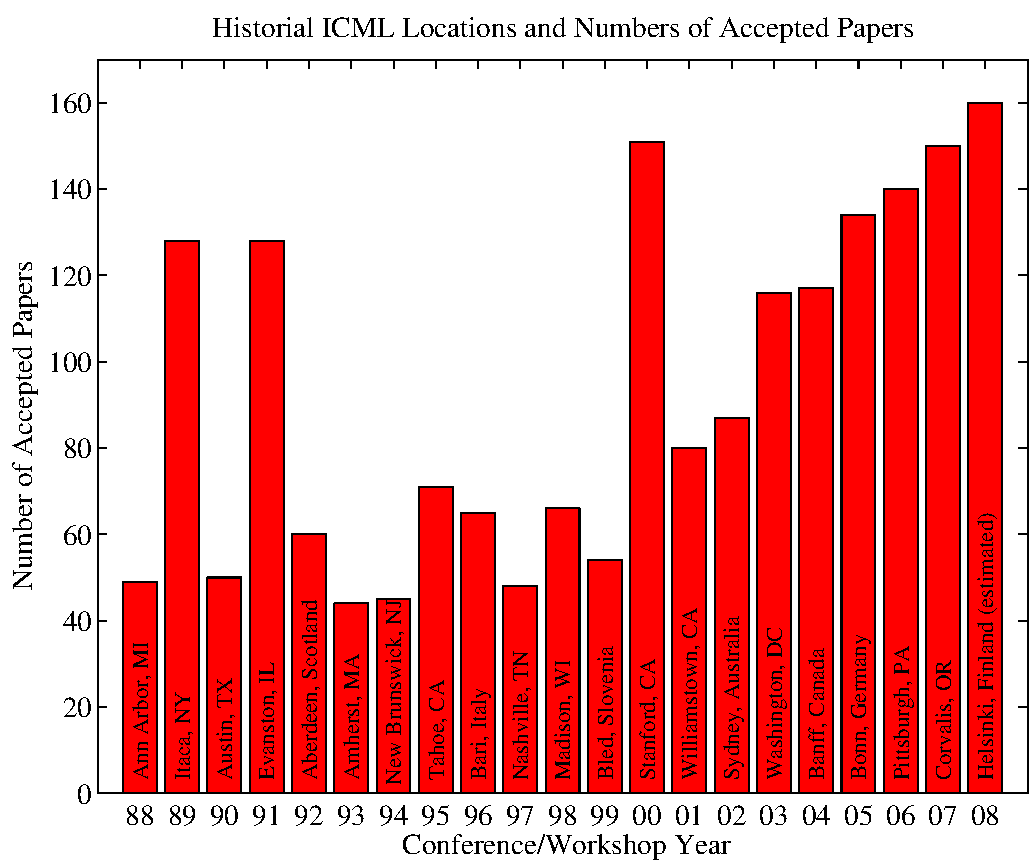
\includegraphics[width=\columnwidth]{icml_numpapers}}
\caption{Historical locations and number of accepted papers for International
  Machine Learning Conferences (ICML 1993 -- ICML 2008) and
  International Workshops on Machine Learning (ML 1988 -- ML
  1992). At the time this figure was produced, the number of
  accepted papers for ICML 2008 was unknown and instead estimated.}
\label{fig:sample-graph}
\end{center}
\vskip -5mm
\end{figure} 

\begin{table}[tb]
\vskip 3mm
\begin{center}
\begin{small}
\begin{sc}
\begin{tabular}{lcccr}
\hline
\abovespace\belowspace
Data set & Naive & Flexible & Better? \\
\hline
\abovespace
Breast    & 95.9$\pm$ 0.2& 96.7$\pm$ 0.2& $\surd$ \\
Cleveland & 83.3$\pm$ 0.6& 80.0$\pm$ 0.6& $\times$\\
Glass2    & 61.9$\pm$ 1.4& 83.8$\pm$ 0.7& $\surd$ \\
Credit    & 74.8$\pm$ 0.5& 78.3$\pm$ 0.6&         \\
Horse     & 73.3$\pm$ 0.9& 69.7$\pm$ 1.0& $\times$\\
Meta      & 67.1$\pm$ 0.6& 76.5$\pm$ 0.5& $\surd$ \\
Pima      & 75.1$\pm$ 0.6& 73.9$\pm$ 0.5&         \\
\belowspace
Vehicle   & 44.9$\pm$ 0.6& 61.5$\pm$ 0.4& $\surd$ \\
\hline
\end{tabular}
\end{sc}
\end{small}
\caption{Classification accuracies for naive Bayes and flexible 
Bayes on various data sets.}
\label{tab:sample-table}
\end{center}
\vskip -3mm
\end{table}



\section{Discussion}
Your discussion should interpret the results, both in terms of summarising the outcomes of a particular experiment, and attempting to relate to the research question(s) which motivated the experiments. For instance, your discussion could start as - "From the experimental results as shown in Fig X and Fig Y, we observe that applying XYZ solution has a positive effect on the test accuracy and achieving a stable learning curve. This is because the XYZ solution does ... " A good report would have some analysis, resulting in an understanding of why particular results are observed, perhaps with reference to the literature. Use bibtex to organise your references -- in this case the references are in the file \verb+example-refs.bib+.  Here is a an example reference \citep{langley00}.  

A good report will relate the results to  published work which can help to give a better understanding of your work -- related approaches, other work on the same data, ideas for future work. 


\section{Conclusions}
\label{sec:concl}
The conclusions section should concisely summarise what you have learned from the experiments you carried out, and relate the findings of your work to the  research questions you posed at the start. Here's a brief example of how you could begin your conclusion - "In this report, we explore the optimization problems in training deep CNN architectures due to XYZ problems. We show the benefits of the proposed solution to this problem by ... . In future, we would like to gain further insights into the solution and/or problem by ..."  It is good if the conclusion from one experiment influenced what you did in later experiments -- your aim is to learn from your experiments.   


A good conclusions section would also include a further work discussion, building on work done so far, and referencing the literature where appropriate.

\bibliography{example-refs}

\end{document} 

